% =================================================================
\documentclass[ 10pt, xcolor = dvipsnames]{beamer}
\usepackage{ beamerthemesplit, lmodern}
\usetheme{Madrid}
\usecolortheme[named=Brown]{structure}
\useinnertheme{rectangles}
\setbeamertemplate{frametitle continuation}{}
\beamertemplatenavigationsymbolsempty
\usepackage{../../../macros-general}
\usepackage{../../../macros-beamer}
\AtBeginSection[]
{
\begin{frame}
\frametitle{Contenido del Tema}
\tableofcontents[ currentsection, sectionstyle = show/shaded, subsectionstyle = show/show/hide]
\end{frame}
}
\AtBeginSubsection[]
{
\begin{frame}
\frametitle{Contenido del Tema}
\tableofcontents[ currentsection, currentsubsection, sectionstyle = show/shaded, subsectionstyle = show/shaded/hide]
\end{frame}
}

\graphicspath{{./figures/}}

% =================================================================
\title[Control Systems]{Control Systems Engineering (EYAG-1005) }
\author[L. I. Reyes-Castro]{Luis I. Reyes-Castro}
\institute[ESPOL]{\normalsize Escuela Superior Polit\'ecnica del Litoral (ESPOL) \\ Guayaquil - Ecuador}
\date[2017-T1]{2017 - First Term}

% -----------------------------------------------------------------
\begin{document}
\begin{frame}[noframenumbering]
\titlepage
\end{frame}
\begin{frame}[noframenumbering]
\frametitle{\shorttitle}
\tableofcontents[ subsectionstyle = hide]
\end{frame}


% =================================================================
\section{Mechanical Systems}

% =================================================================
\section{Electric Circuits}

% =================================================================
\section{Armature-controlled DC Motors}

% -----------------------------------------------------------------
\begin{frame}[allowframebreaks]
\frametitle{\insertsection}

The model for the armature-controlled DC motor involves both an electric circuit an a rotational mechanical system. \textbf{If no load is attached to the armature} \linebreak then the models are as shown below: 
\halfskip

\begin{figure}[htb]
\centering
\def\svgwidth{0.9\columnwidth}
\input{figures/motor-dc_armadura.eps_tex}
\end{figure}

\end{frame}

% -----------------------------------------------------------------
\begin{frame}[allowframebreaks]
\frametitle{\insertsection}

\begin{columns}

\begin{column}{0.45\textwidth}
\textbf{Example \\ (Nise, Problem 2.46*):}
\halfskip

Consider the mechanism on the right, where an armature-controlled DC motor drives a block of mass by means of a system of gears. The input is the supplied voltage $e_a(t)$ and the output is the displacement of the block of mass $x(t)$. 
\halfskip

Find the transfer function:
\[
G(s) \, = \, \frac{X(s)}{E_a(s)}
\]

\end{column}

\begin{column}{0.45\textwidth}
\begin{figure}[htb]
\centering
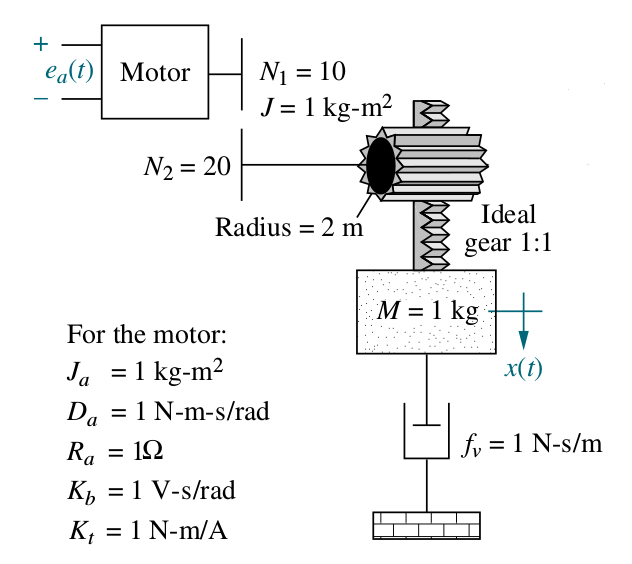
\includegraphics[width=\columnwidth]{figures/nise_prob-2-46.jpeg}
\end{figure}
\fullskip
{
\small
\textbf{Note:} Each of the three gears shown has moment of inertia $J = 1$ kg-m\tsup{2}. 
}

\end{column}

\end{columns}
\framebreak

Electric circuit and equivalent rotational mechanical system: 
\begin{figure}[htb]
\centering
\def\svgwidth{0.9\columnwidth}
\input{figures/nise_prob-2-46.eps_tex}
\end{figure}

\end{frame}

% -----------------------------------------------------------------
\begin{frame}[allowframebreaks]
\frametitle{\insertsection}

Models: 
\begin{itemize}
\item Electric circuit:
\[
e_a(t) \, = \, R_a \, z_a(t) + K_b \, \dot{\theta}_1(t)
\]
\item Rotational mechanical system:
\begin{align*}
& ( J_a + J ) \, \ddot{\theta}_1(t) + ( 2J + J_2 ) \, \ddot{\theta}_2(t) 
\, = \, K_t \, z_a(t) - D_a \, \dot{\theta}_1(t) - D_2 \, \dot{\theta}_2(t) \\[1ex]
& N_1 \, \theta_1(t) \, = \, N_2 \, \theta_2(t) \\[1ex]
& x(t) \, = \, r \, \theta_2(t)
\end{align*}
\end{itemize}
\framebreak

Taking the Laplace Transform of both equations on both sides: 
\begin{itemize}
\item Electric circuit:
\[
E_a(s) \, = \, R_a \, Z_a(s) + K_b \, s \, \Theta_1(s)
\]
\item Rotational mechanical system:
\begin{align*}
& ( \, ( J_a + J ) \, s^2 + D_a \, s \, ) \, \Theta_1(s) + 
( \, ( 2J + J_2 ) \, s^2 + D_2 \, s \, ) \, \Theta_2(s) 
\, = \, K_t \, Z_a(s) \\[1ex]
& \Theta_1(s) \, = \, ( N_2/N_1 ) \, \Theta_2(s) \\[1ex]
& \Theta_2(s) \, = \, (1/r) \, X(s)
\end{align*}
\end{itemize}
\framebreak

Solving...
\begin{itemize}
\item Armature current:
\[
Z_a(s) \, = \, \frac{ E_a(s) - K_b \, s \, \Theta_1(s) }{R_a}
\]
\item Angles in terms of displacements:
\[
\Theta_1(s) \, = \, \left( \frac{N_2}{N_1 \, r} \right) X(s) \qquad \qquad
\Theta_2(s) \, = \, \left( \frac{1}{r} \right) X(s)
\]
\item Sum of torques equation: 
\begin{align*}
& ( \, ( J_a + J ) \, s^2 + D_a \, s \, )\left( \frac{N_2}{N_1 \, r} \right) X(s) + 
( \, ( 2J + J_2 ) \, s^2 + D_2 \, s \, ) \left( \frac{1}{r} \right) X(s) \\
& = \, \left( \frac{K_t}{R_a} \right) \, \left[ \, E_a(s) - K_b \left( \frac{N_2}{N_1 \, r} \right) s \, X(s) \, \right]
\end{align*}
\framebreak
\item Sum of torques equation (continued):
\begin{align*}
& \frac{1}{r} \, \left[ \,
\left( \frac{N_2 \, ( J_a + J )}{N_1} + 2J + J_2 \, \right) s^2 + 
\left( \frac{N_2 \, ( D_a + K_t K_b / R_a )}{N_1} + D_2 \, \right) s \, \right] X(s) \\
& = \, \left( \frac{K_t}{R_a} \right) E_a(t)
\end{align*}
\item Finally:
\begin{align*}
& G(s) \, = \,
\frac{ \frac{r \, K_t}{R_a} }{
\left( \frac{N_2 \, ( J_a + J )}{N_1} + 2J + J_2 \, \right) s^2 + 
\left( \frac{N_2 \, ( D_a + K_t K_b / R_a )}{N_1} + D_2 \, \right) s } \\
& \Longrightarrow \, G(s)
\, = \, \frac{1}{ 5 s^2 + 4s } 
\, = \, \frac{1/5}{ s^2 + (4/5)s } 
\, = \, \frac{1/5}{ s \, ( \, s + (4/5) \, ) }
\end{align*}
\end{itemize}

\end{frame}

% =================================================================
\section{Aerospace Vehicles}

% -----------------------------------------------------------------
\begin{frame}[allowframebreaks]
\frametitle{\insertsection}

Model of a simple 2D wing with elevator:
\begin{figure}[htb]
\centering
\def\svgwidth{0.9\columnwidth}
\input{figures/simple-wing.eps_tex}
\end{figure}

\end{frame}

% -----------------------------------------------------------------
\begin{frame}[allowframebreaks]
\frametitle{\insertsection}

Model of a \textbf{puller-configuration} fixed-wing aircraft: 
\begin{figure}[htb]
\centering
\def\svgwidth{\columnwidth}
\input{figures/drone-puller.eps_tex}
\end{figure}

\end{frame}

% -----------------------------------------------------------------
\begin{frame}[allowframebreaks]
\frametitle{\insertsection}

Model of a \textbf{pusher-configuration} fixed-wing aircraft: 
\begin{figure}[htb]
\centering
\def\svgwidth{\columnwidth}
\input{figures/drone-pusher.eps_tex}
\end{figure}

\end{frame}

\end{document}
